% !TeX root = ../../../main.tex
\begin{figure}[htbp]
\begin{ChEightFloatBody}

    \centering
    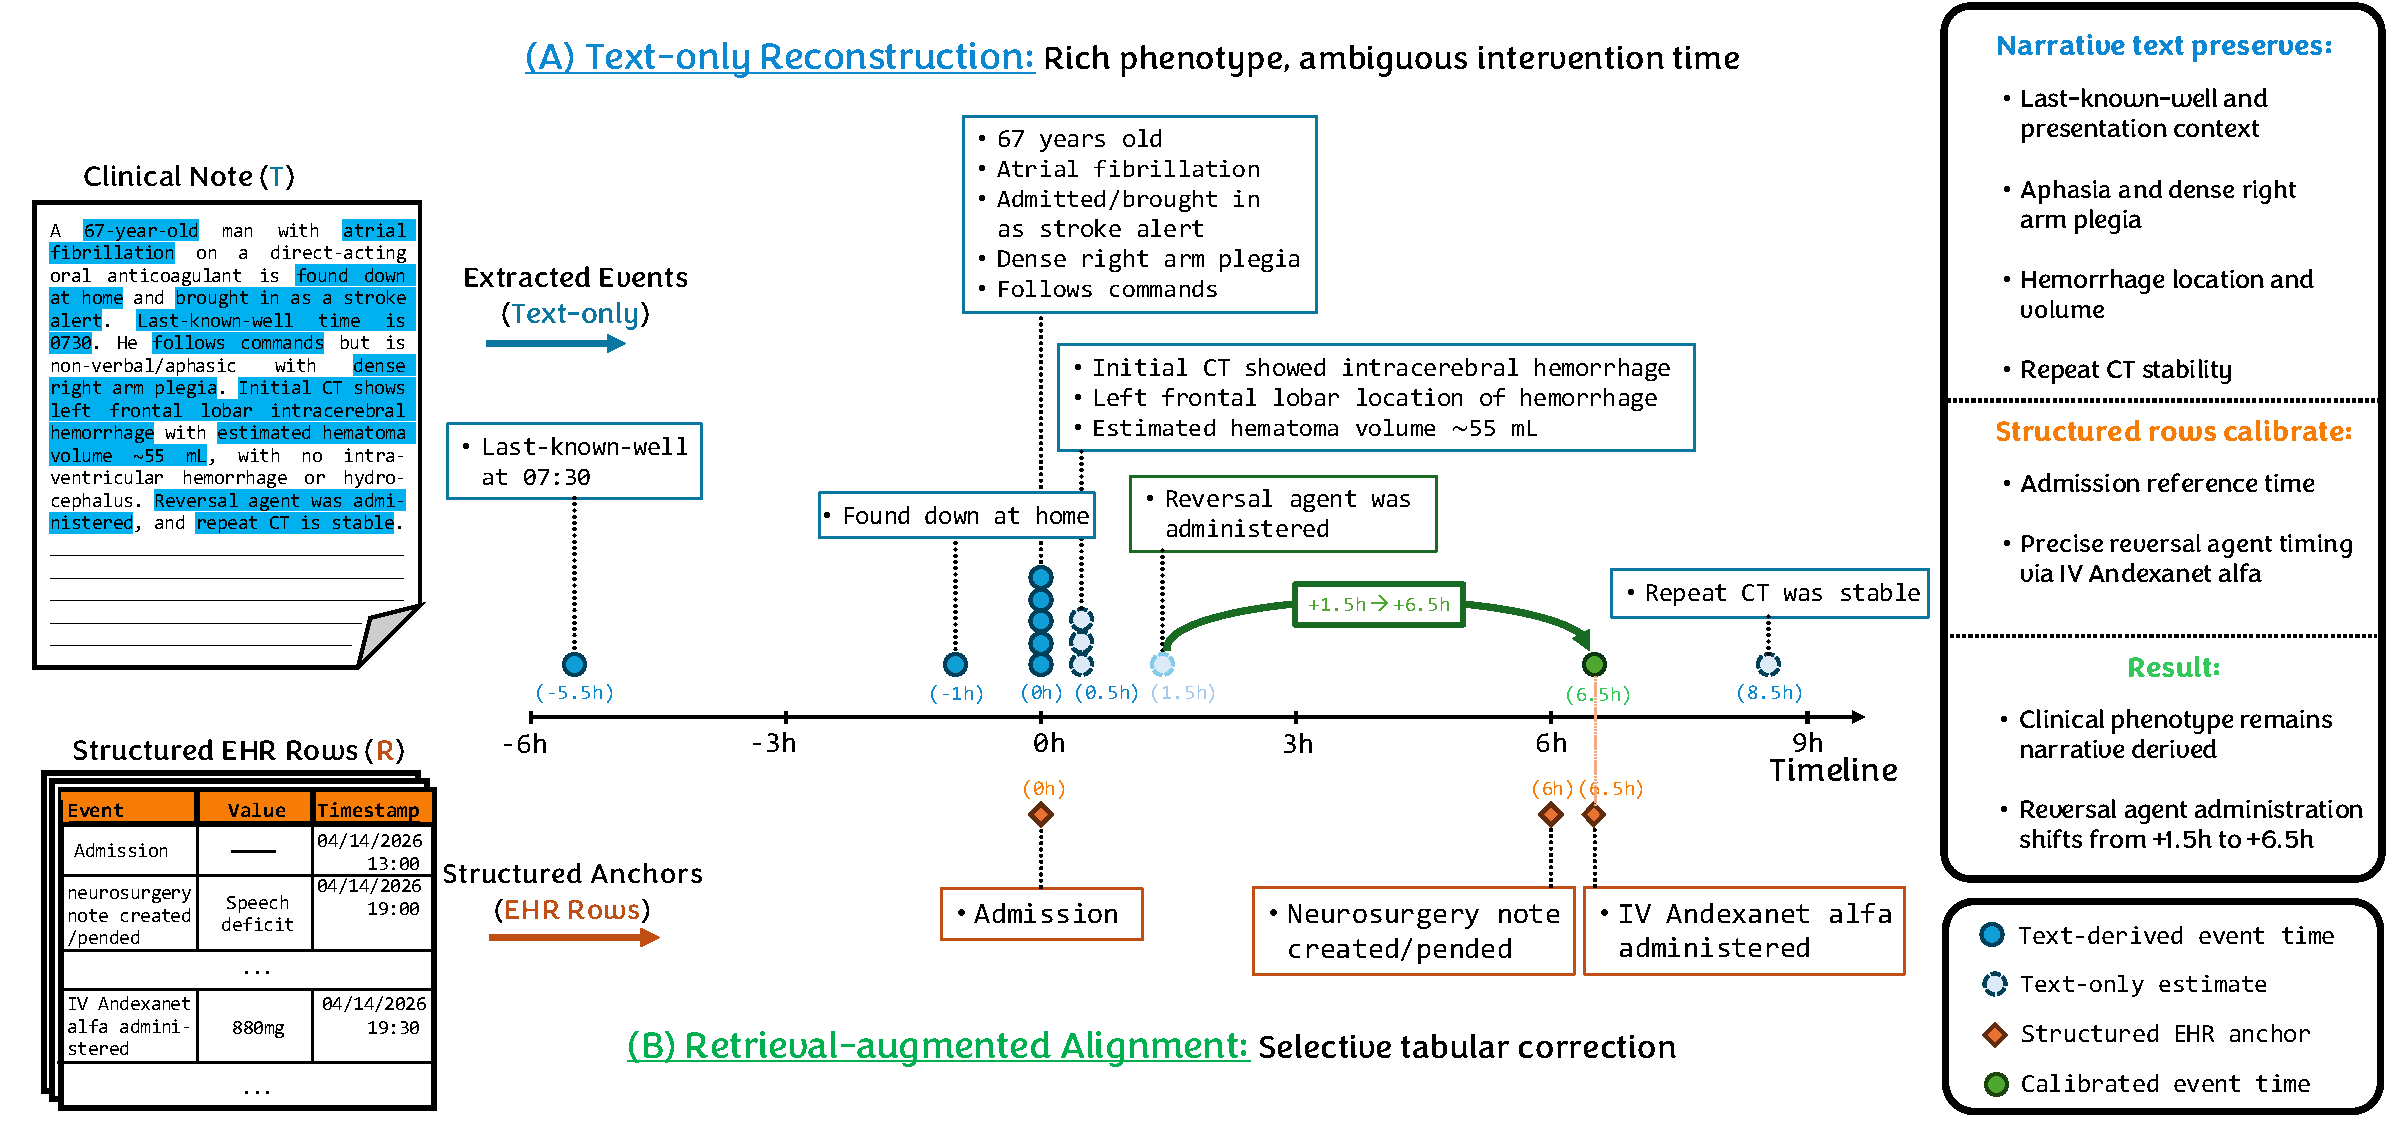
\includegraphics[width=0.85\textwidth]{Chapters/chapter-08/images/plots/TTA-Overview-Figures-PSB.pdf}
    
    
    
    

\end{ChEightFloatBody}
\caption{
    \ChEightRebuttal{Motivation for retrieval-augmented temporal grounding using a synthetic stroke-alert case constructed for illustration.}
    (\textbf{A}) Text-only reconstruction can recover clinically meaningful narrative events, but intermediate event times may remain ambiguous.
    (\textbf{B}) Retrieved structured EHR rows provide partial temporal evidence that can calibrate text-derived events when clinically relevant, improving temporal placement while preserving narrative event content.
    }\ChEightFloatLabel{ch08:fig:motivation_multimodal_alignment}
\end{figure}